\chapter{Mathematical and technical Fundamentals}
\label{chap:mathFund}

\section{Synthetic aperture focusing technique (SAFT)}
\label{sec:SAFT}
The \ac{saft} is used to restore images from raw data of ultra sonic imaging techniques.
By combining the data of \acp{ascan} from a multitude of emitter-receiver combinations it is possible to reconstruct an high resolution image.

Figure \ref{ascan_example} shows the principle of an \ac{ascan}. The 3D-volume of the aperture is shown on the left side. For this example only two of the many transducers that normally are placed on the wall of the aperture are shown. On the right the plot of the pressure is shown by the graph. The actual \ac{ascan} consists of a discrete plot of the transition of the pressure at that receiving transducer where the pressure $p(t)$ is plotted over the time $t$. The first pulse in the graph is the transmission pulse that reaches the receiving transducer without much interaction of the pressure wave with matter. The second pulse originates after the first pressure wave scatters at a certain location in the tissue and has a lower amplitude than the first pulse. The amount of time it takes for the pulse to propagate from the emitter to the point of scattering and then to the receiving transducer is called \ac{tof}. The reason for the decreased amplitude of the reflected pulse compared to the transmission pulse is the longer path that the wave has to travel and as a consequence thereof the higher attenuation leads to the lower amplitude. 


\begin{figure}[H]
    \centering
    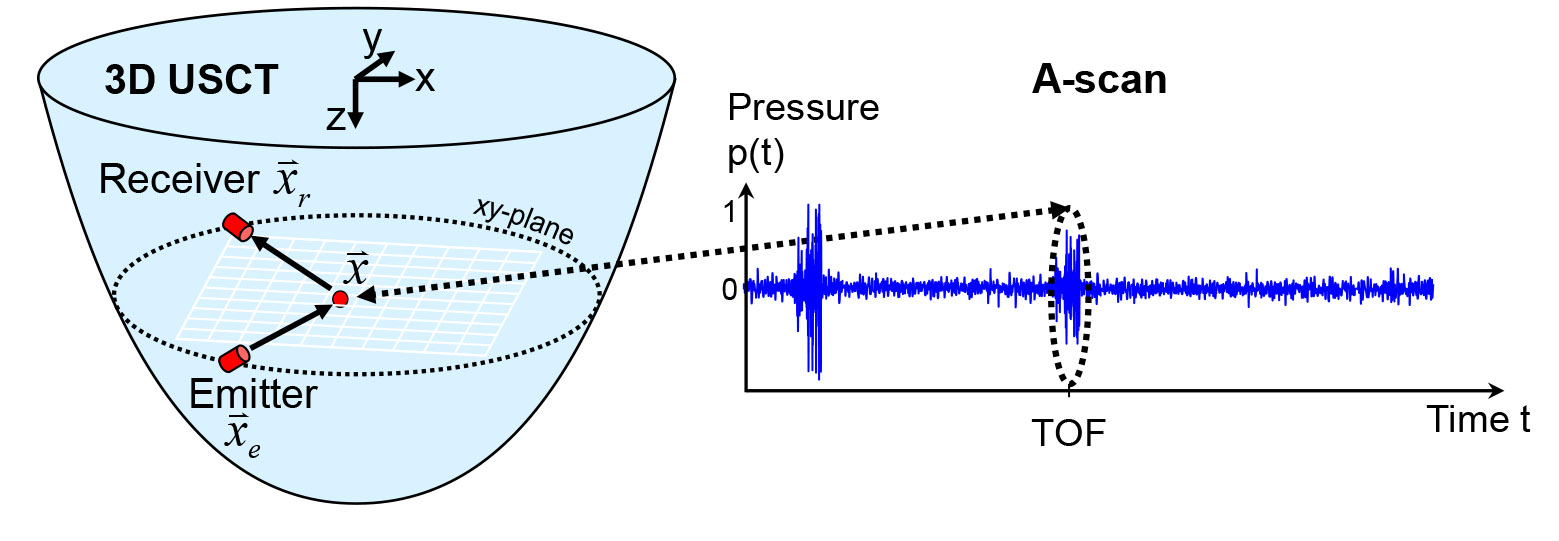
\includegraphics[width=1\textwidth]{GPU_based_3D_SAFT_reconstruction_including_phase_aberration-4.jpg}
    \caption{ Simple example of an \ac{ascan} for one emitter-reciever combination. One transducer $\overrightarrow{\chi_e}$ emits a pulsed wave-front into the aperture. The \ac{ascan} shows the pressure over the time measured by the receiving transducer $\overrightarrow{\chi_r}$. The first pulse in the diagram is the pulse cause by the transition of the emitted wave-front. The second pulse is from the reflection on an object in the aperture. Picture source: \cite{Kretzek2014GPUAberration}. }
    \label{ascan_example}
\end{figure}

There are two principal ways to reconstruct an image from a set of \acp{ascan} using the \ac{saft} which both yield quite a similar result but differ in the computation costs. Each voxel eventually gets assigned a certain value which corresponds to the intensity of that voxel in the final image. 

\bigskip

For the first method one starts with the desired voxel that the value should be calculated of.
A simple 2D-example of the xy-plane from figure \ref{ascan_example} is shown in figure \ref{SAFT_explain1}. On the left is the aperture with the 3D-volume shown as a 2D grid. The emitter $e_i$ and the two receiving transducers $r_j$ and $r_{j+1}$ are on the outer shell of the aperture. On the right two \acp{ascan} are depicted. The upper \ac{ascan} shows the plot of the pressure of the configuration where emitter $e_i$ transmits a wave-front and $r_j$ measures the transition of the pressure. The plot below is for emitter $e_i$ but this time with transducer $r_{i+1}$ receiving. Considering how close $r_j$ and $r_{j+1}$ are placed to each other in this example the \ac{ascan} on the bottom shows an rather exaggerated negative time shift compared to the \ac{ascan} above.

\begin{figure}[H]
    \centering
    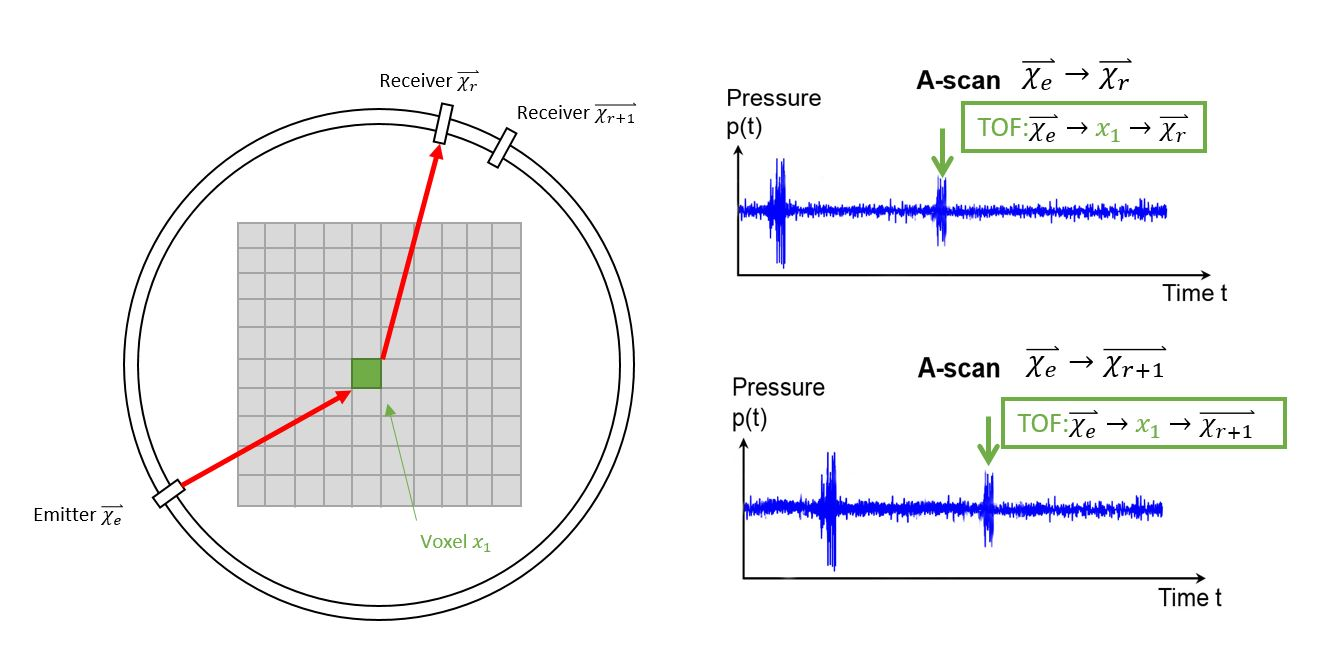
\includegraphics[width=1\textwidth]{SAFT_explaination1.jpg}
    \caption{Basic principle of the \ac{saft}. For one voxel every \ac{ascan} is analysed at a certain \ac{tof}. The final voxel value is the sum of every amplitude at the time in each corresponding \ac{ascan}. The procedure has to be repeated for each individual voxel. }
    \label{SAFT_explain1}
\end{figure}


If we know the location of our voxel in our plane then we can calculate the \ac{tof} from each emitter to each receiving transducer. For this basic example the equation \ref{eqation_tof} shows how to calculate the \ac{tof} for the first voxel when neglecting the different speeds of sound in for the different types of tissue.

\begin{equation}
TOF_{1,ij} =  \frac{dist_{e_i,x_1} + dist_{x_1,r_{j}} }{ SOS } 
\label{eqation_tof}
\end{equation}

$dist_{e_i,x_1}$ corresponds to the euclidean distance of the emitter $e_i$ to the desired voxel $x_1$ and $dist_{x_1,r_{j}}$ analogously to the euclidean distance from the voxel to the receiver.
The speed of the sound wave is considered by $SOS$ in the equation.

The \ac{tof} for the first emitter-receiver combination is shown a the green arrow in the upper \ac{ascan} in figure \ref{SAFT_explain1}. By accident the \ac{tof} is directly located at the peak of the reflected wave-front. To determine the corresponding sample in the discrete \ac{ascan} either a linear 1D-interpolation between the two samples left and right of the \ac{tof} can be performed. Otherwise a nearest neighbour interpolation can yield a viable time sample.
For this \ac{tof} the amplitude of the \ac{ascan} then is taken and added to the voxel value of voxel $x_1$. 
In the same manner the \ac{tof} of the second receiver-emitter configuration is calculated and a viable sample in the \ac{ascan} can be found. In this case the sample is not located at the peak of \ac{ascan} anymore. As well, for that time sample the value of the \ac{ascan} is added to the voxel value for $x_1$ even though it is considerably lower than before and does not influence the final voxel value that much. 
This procedure is repeated for every emitter-receiver combination and every aperture rotation shift so that the final result is the voxel value only for voxel $x_1$.
To reconstruct the whole 3D image these steps have to be repeated for every voxel in the volume.

Equation \ref{eqation_Voxel_value} shows the calculations necessary to get the voxel value $V_k$ for an arbitrary voxel $k$. 
\begin{equation}
V_k = \sum_{i}^{N_e}\sum_{j}^{N_r} A(TOF_{k,ij}) = \sum_{i}^{N}\sum_{j}^{N} A \left (\underset{ = TOF_{k,ij} } {\underbrace{\frac{ dist_{e_i,x_k} + dist_{x_k,r_{j}}}{SOS} }}  \right )
\label{eqation_Voxel_value}
\end{equation}

For $N$ transducers the reconstructed value $V$ of each voxel $k$ consists of the sum of each pressure values at the \ac{tof} in the respective \acp{ascan} for all emitter-receiver combinations ($N_e, N_r$). 

\bigskip

For the second possibility to reconstruct an image from the raw data we do not start at a certain voxel but look at each individual \ac{ascan}. In figure \ref{SAFT_explain2} the \ac{usct} aperture is shown this time with only one emitter-receiver configuration. On the right side the \ac{ascan} for this configuration is schematically plotted.

\begin{figure}[H]
    \centering
    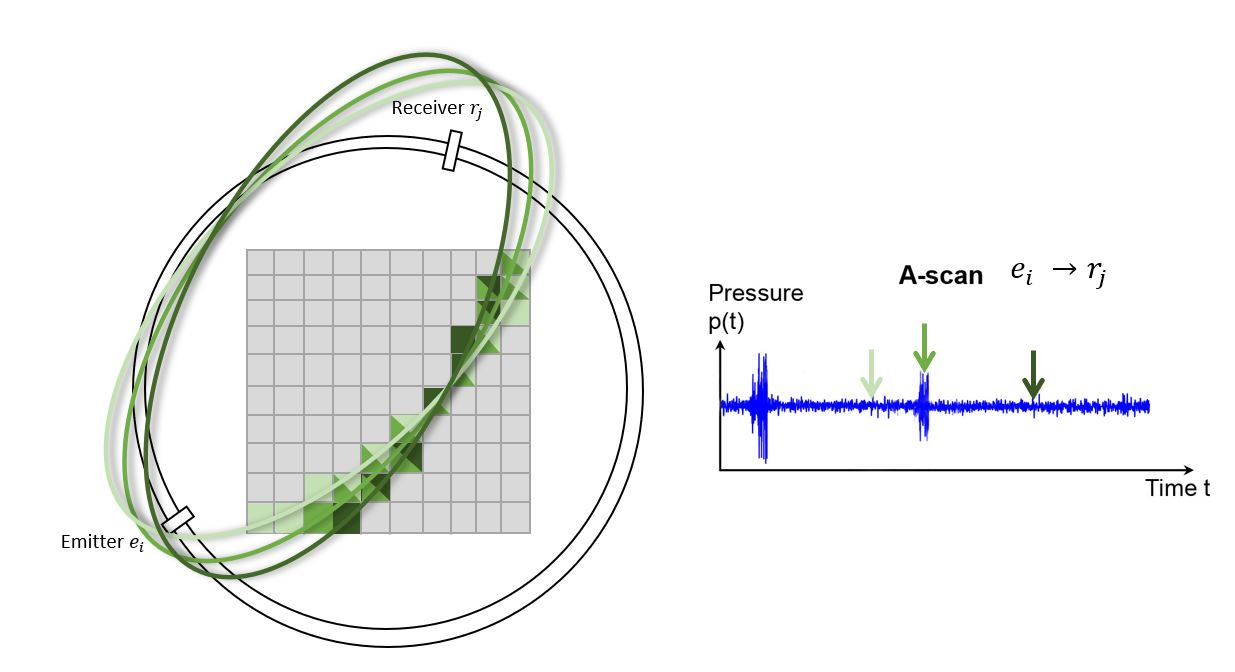
\includegraphics[width=1\textwidth]{SAFT_explaination2.jpg}
    \caption{ Alternative method to reconstruct the image for the \acp{ascan}. }
    \label{SAFT_explain2}
\end{figure}


In contrast to the first method we do not only pick one certain sample in the \ac{ascan} but a few. 
Theoretically one could use every sample in the \ac{ascan} to reconstruct the image, however is not recommendable as this would require a long time to compute. In general it is advisable to pick at least one sample at location of the maximum peak that is caused by the scattering of the wave front at the location of one voxel. In this example three samples are chosen marked by the arrows in the different shades of green. By choosing one sample in the \ac{ascan} we avoid having to interpolate during this step.
With these three chosen \acp{tof} in one \ac{ascan} and the location of the emitter and receiver it is not possible to determine only one voxel to add the amplitude values to. For one emitter-receiver combination and one certain \ac{tof} a multitude of voxels are eligible to be the source of the scattering. To be precise an eclipse covers every possible scattering location where the \ac{tof} from emitter $e_i$ to receiver $r_j$ is equal to the chosen \ac{tof} from the \ac{ascan}. For each of the three chosen \acp{tof} there is one eclipse in figure \ref{SAFT_explain2}. Along those eclipses to every voxel which is cut by the eclipse the amplitude value is added to. This is schematically shown by the different shapes of the squares beneath each eclipse. A single colour means, that to that voxel only one value was added. Analogously do two or even three colours indicate, that multiple pressure values are added to that voxels value. 
Bresenham's line drawing algorithm \cite{Bresenham2010AlgorithmPlotter} is used to decide which set of voxels approximates the eclipse best and therefore to which voxel the corresponding amplitude value is added. To find the suitable coordinates of each voxel an interpolation in 3D has to be performed.
This procedure leads to the fact, that many voxels get assigned pressure values even though they were not at the location of the scattering. However, when this procedure is repeated for every \ac{ascan} ultimately those voxels that are actually at the true location of the scattering will be part of so many eclipses that their final voxel value will be a lot higher than the surrounding noise. By superposing the voxel values the surrounding noise is negligible and does not affect the final image. An example is shown in figure \ref{eclipse_super}.


\begin{figure}[H]
    \centering
    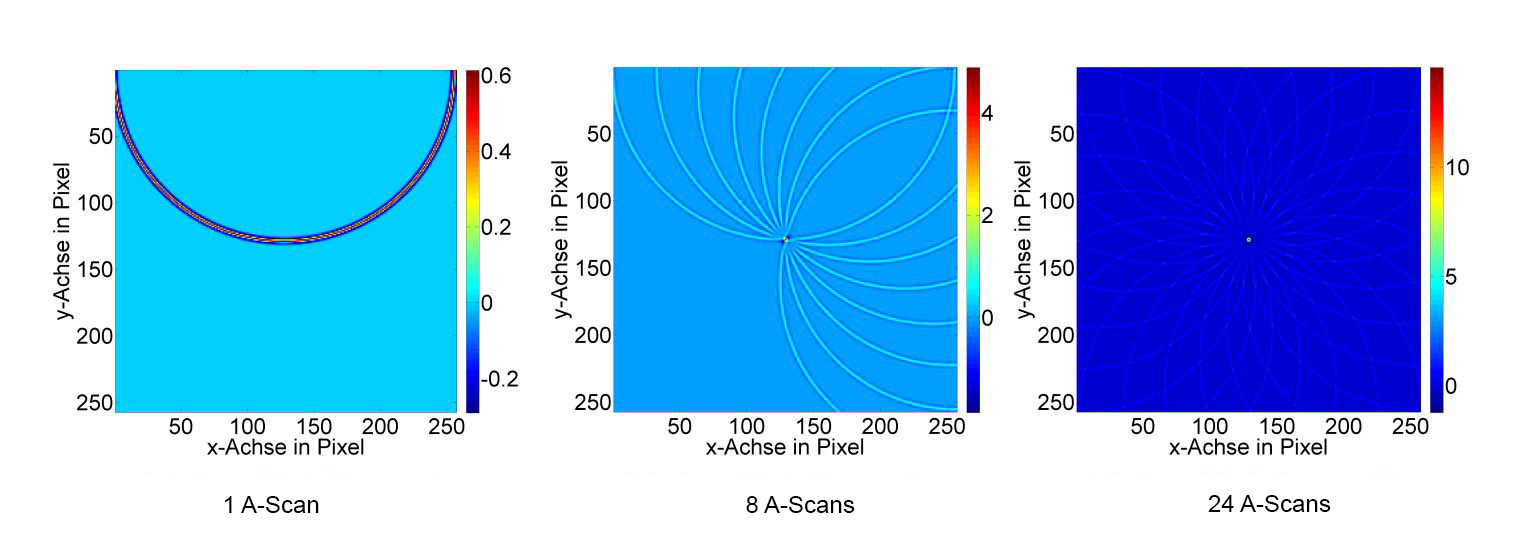
\includegraphics[width=1\textwidth]{eclipse_superposition_hucker.jpg}
    \caption{ Superposition of multiple eclipses during the reconstruction of the final image. By averaging the voxel values of multiple eclipses each eclipse loses significance in the final image.
    Image Source: \cite{PatrickHucker2014EvaluationRuckstreumodells}}
    \label{eclipse_super}
\end{figure}


For only one \ac{ascan} the value of only that one \ac{tof} of the \ac{ascan} is added to each voxel along the eclipse. Therefore, the eclipse is very prominent in the left-most pane of figure \ref{eclipse_super}. In the plot in the middle there are already eight different \acp{ascan} used. Each eclipse is still distinguishable but lost opacity nonetheless.
In the pane on the right side 24 \acp{ascan} are superimposed. At the point of the intersection of all 24 eclipses one single pixel has a rather high value whereas the surrounding eclipses are barely visible anymore. There more \acp{ascan} are used for the reconstruction the higher the contrast of the final image gets.

\bigskip

Both methods have their advantages and disadvantages. However, during this thesis the first reconstruction algorithm was used. One of the main reasons for that is that all the calculations are easily calculable in parallel and therefore profit from the high number of parallel threads on the GPU architecture. Furthermore, as was mentioned that the eclipse method makes multiple interpolations for each voxel in 3D necessary whereas the first method only interpolates in 1D between two sample values. So, by choosing the first method very expensive computation operations can be avoided.


Currently the reconstruction of a clinical relevant volume of 1024x64 voxels and 1.7 million of A-scans takes about 23 minutes \cite{Kretzek2014GPUAberration}.






\section{3D-USCT}

The three dimensional ultra sonic computed tomography (3D-USCT) imaging technique is a promising rather new technique for the detection of breast cancer in early stages \cite{Ruiter2011RealizationUSCT}.

The second version prototype of the 3D-\ac{usct} can be seen in figure \ref{usct_example}. On the left the picture shows the patient bed with the aperture for the breast. The patient has to lie down on their stomach during the imaging procedure. The breast will be placed in the water-filled semi-ellipsoidal aperture which can be seen on the lower right side of the figure. On the top-right of figure \ref{usct_example} the aperture is visible with over 2000 US-transducers.
For the examination the patient has to lie down on a bed with an semi-ellipsoidal aperture for the breasts and has to remain still to avoid image degradation \cite{Ruiter2011RealizationUSCT}. 

To measure the pressure over time the prototype of the \ac{usct} at the KIT comprises 628 emitting and 1413 receiving transducers fitted into the wall of the aperture. The aperture itself has a height of 17cm and diameter of 26cm \cite{Kretzek2014GPUAberration}.

During the scan the breasts are immersed in the aperture which is filled with water as coupling medium for the ultrasound measurement. During the measurement for every emitter-receiver-combination an \ac{ascan} is recorded. 

From these data it is possible to reconstruct a picture of the breast tissue. For the reconstruction of the image the \ac{saft} is used.
Three modalities for the image reconstruction are currently in use: reflectivity, speed of sound and attenuation \cite{Jirik2012Sound-speedTomography}.
With these three modalities it is possible to reconstruct an image with a submillimetre-resolution.


During each scan one transducer acts as an emitter whereas all the other transducers are receiving the signal. For every emitter-receiver combination a so called \ac{ascan} is recorded. Each \ac{ascan} comprises the progression of the pressure at the transducer which is plotted over the time. After each emitter-receiver combination was recorded the aperture is rotated to compensate the gaps between each \ac{tas}. In total there are ten positions for which each emitter-receiver scan is repeated.
 


\begin{figure}[H]
    \centering
    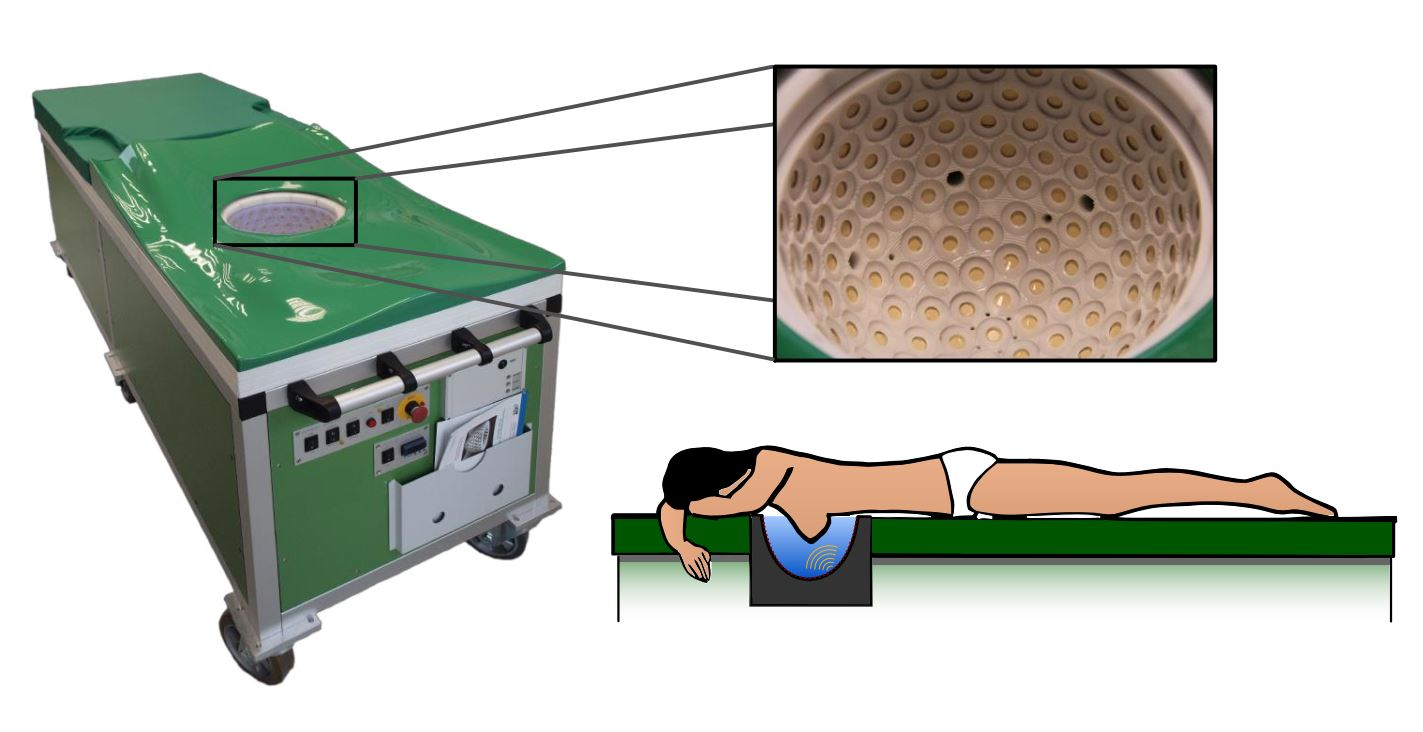
\includegraphics[width=1\textwidth]{usct_schematic.jpg}
    \caption{The prototype of an 3D-\ac{usct} at the KIT research facility. Picture source: \cite{Kretzek2014GPUAberration}. }
    \label{usct_example}
\end{figure}


For the generation of the final image so far three different modalities are used. 


- aperture rotation -> sparseness -> more data

- data processing




\section{Characterisation of reflections}

During the acquisition of the data each emitting transducer emits a wave-front into the aperture which then interacts with the breast tissue in a distinct way. Therefore, it is important to take into consideration how the sonic wave interacts and scatters at the surface of the different tissue types and other objects in the aperture. The directional information of the reflections are lost during the classical approach of the \ac{saft} \cite{Kretzek2015EvaluationTomography}. As this thesis is focused on the tissue classification based on a back scattering model the reflection characteristics of the tissue can no longer be neglected. Figure \ref{fig:types_of_reflect} shows four different kinds of scattering and reflection depending on the structure of the surface and the direction of the incident sonic pulse.

\begin{figure}[H]
     \centering
     \begin{subfigure}[b]{0.23\textwidth}
         \centering
        \fbox{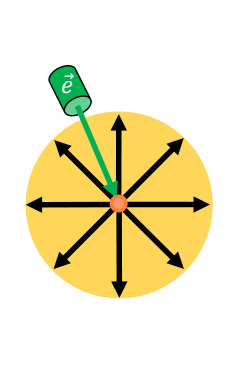
\includegraphics[width=0.8\linewidth]{ReflectionCharacteristics_IUS2015-1.jpg}}
         \caption{Isotropic scattering at point source.}
         \label{fig:reflect_isotropic}
     \end{subfigure}
     \hfill
     \begin{subfigure}[b]{0.23\textwidth}
         \centering
         \fbox{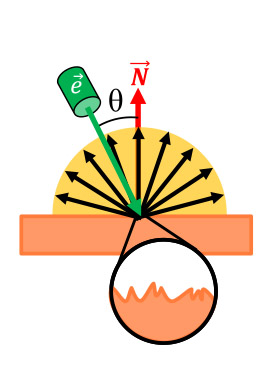
\includegraphics[width=0.87\textwidth]{ReflectionCharacteristics_IUS2015-2.jpg}}
         \caption{Diffuse scattering on rough surface.}
         \label{fig:reflect_diffuse}
     \end{subfigure}
     \hfill
     \begin{subfigure}[b]{0.23\textwidth}
         \centering
         \fbox{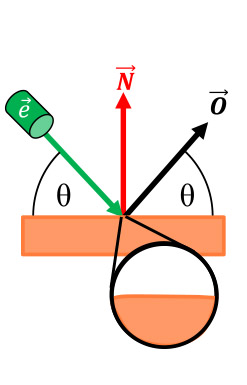
\includegraphics[width=0.8\textwidth]{ReflectionCharacteristics_IUS2015-3.jpg}}
         \caption{Specular reflection on a glossy surface.}
         \label{fig:reflect_specular}
     \end{subfigure}
     \hfill
     \begin{subfigure}[b]{0.23\textwidth}
         \centering
         \fbox{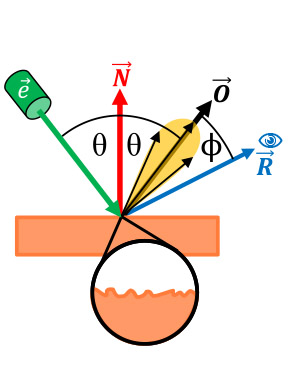
\includegraphics[width=0.93\textwidth]{ReflectionCharacteristics_IUS2015-4.jpg}}
         \caption{Specular reflection and diffuse reflection.}
         \label{fig:reflect_mixed}
     \end{subfigure}
        \caption{Reflection characteristics of different surfaces and angle of incidence. Picture source: \cite{Kretzek2015EvaluationTomography}}
        \label{fig:types_of_reflect}
\end{figure}


Figure \ref{fig:reflect_isotropic} shows the principle of isotropic scattering at a dot-like scattering point. Transducer $\overrightarrow{e}$ emits a sound-wave into the volume. When the sound wave reaches the point of scatter it will be reflected homogeneously into every direction with an isotropic distribution of intensity. This emitted concentrical spherical wave has a constant energy distribution in each direction. This is a theoretical principle of a reflection which the \ac{saft} is based on since it neglects all direction information of the received sound wave.

A more realistic scattering model can be seen in figure \ref{fig:reflect_diffuse}. The diffuse scattering occurs on a rough and matt surface where the incoming energy of the sonic wave is equally scattered into every direction above the surface of the material (Lambertian reflectance). The surface of the material then appears to have the same radiance from every angle. The Cosine-Lambert-Law states that the angle of the inciding wave-front has an influence on the the radiated intensity \cite{lambert1892lamberts}.
The smaller the angle $\theta$ between the incoming wave-front and the surface normal $\overrightarrow{N}$, the higher the scattered intensity from the surface. In other words: the diffuse reflection is proportional to the amount of light that hits the surface per unit area \cite{illum_Phong}, which is represented by equation \ref{eq:lambert_cosine}:

\begin{equation}
I_{diffus} \propto cos(\theta)
\label{eq:lambert_cosine}
\end{equation}



\begin{figure}[H]
    \centering
    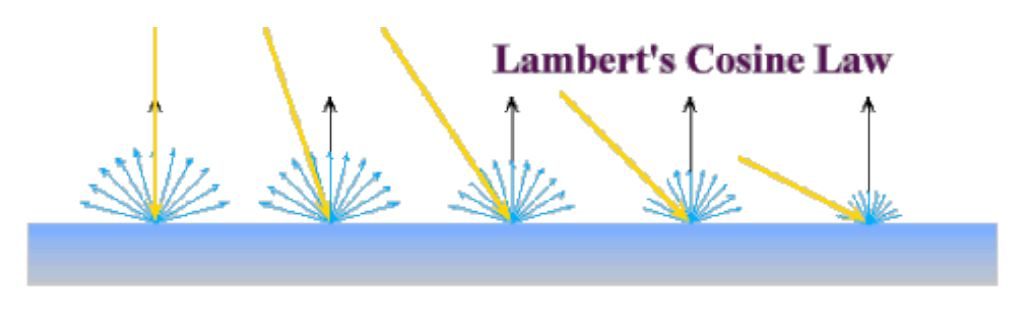
\includegraphics[width=0.75\textwidth]{lambert_cosine.jpg}
    \caption{Representation of the Lambert Cosine Law. The scattered intensity from the surface is proportional to the cosine of the angle between the incoming wave-front and the surface normal. Picture source: \cite{illum_Phong}.}
    \label{Lambert_cosine_law}
\end{figure}


The third reflection characteristic is called specular reflection and can be seen in figure \ref{fig:reflect_specular}. Whereas in the case of the diffuse scattering the energy density of the scattered wave is evenly distributed above the to the emitter facing side of the surface, the specular reflection has a very concentrated direction of emission. For glossy and even surfaces the incoming wave is reflected on the surface whereas the entry angle  $\theta$ is equal to the exit angle $\theta$.
The main reflection direction is described by vector $\overrightarrow{o}$. The closer the receiver vector is to this main reflection direction the higher the received intensity. 
Furthermore, for an ideal specular reflection it is assumed that the energy of the incoming wave-front is equal to the reflected energy from the surface. Since the transducers of the 3D-\ac{usct} emit unfocused ultrasound waves the angle of the incoming sound-wave can not be determined exactly. For the previous work \cite{PatrickHucker2014EvaluationRuckstreumodells} the specular reflection was assumed to be the prevailing model.


Figure \ref{fig:reflect_mixed} shows a combination of specualar reflection and diffuse scattering. This model is appropriate for materials with a surface structure somewhere in-between rough and glossy. The emitted intensity is a mixture between the directly reflected energy based on the specular reflection and the scattered energy of the diffuse scattering model. This results in a cone shaped beam with an opening angle based on the scattering factor of the material. Again, the angle between the inciding wave front and the surfaces normal determines the intensity of the reflected wave. Now also applies that the angle $\Phi$  between the receiver vector $\overrightarrow{R}$ to the main reflection direction $\overrightarrow{o}$ affects the received intensity as well. The smaller $\Phi$ becomes the greater is the measured intensity.







\section{Spherical coordinate system}
Spherical coordinates are used to create an arbitrary amount of normal vectors to characterise the different directions for each voxel. Depending on the available computation power and memory it is possible to create as many normals as possible to cover as many possible directions as possible.


\subsection{Spherical coordinate system in 3D}

In three dimensions the spherical coordinate system consists of a radius $r$, and inclination $\vartheta$ and an azimuth $\varphi$. The conversion from one coordinate systems to the other can be seen in tables \ref{table_pol_to_cart} and \ref{table_cart_to_Pol}.

\begin{figure}[H]
  \centering
  \begin{minipage}[b]{0.45\textwidth}
    \centering
  \fbox{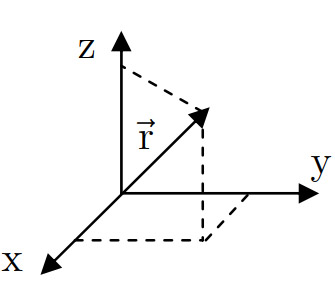
\includegraphics[width=0.75\linewidth]{cartesian_coord.jpg}}
  \caption{Cartesian coordinate system \cite{Prof.Dr.-Ing.GertF.Trommer2013FelderWellen}.}
  \end{minipage}
  \hfill
  \begin{minipage}[b]{0.45\textwidth}
    \centering
  \fbox{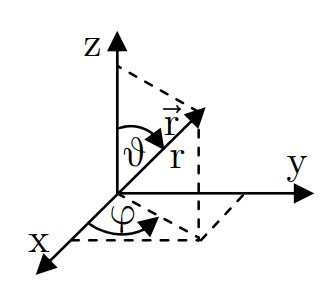
\includegraphics[width=0.75\textwidth]{polar_coord.jpg}}
  \caption{Spherical coordinate system \cite{Prof.Dr.-Ing.GertF.Trommer2013FelderWellen}.}
  \end{minipage}
    \hfill
\label{polar_cart_systems}
\end{figure}




\begin{table}[H]
\centering
\begin{tabular}{|ll|}
\hline
\textbf{Cartesian coordinate system} & \textbf{Spherical coordinate system}                                                                            \\ \hline
$x $                            & $= r \cdot sin(\vartheta) \cdot cos(\varphi)$ \\
$y $                            & $= r \cdot sin(\vartheta) \cdot sin(\varphi)$ \\
$z $                            & $= r \cdot cos(\vartheta)$                                                  \\ \hline
\end{tabular}
\caption{Conversion of polar coordinates to Cartesian coordinates  \cite{Bronstein2005TaschenbuchMathematik}.}
\label{table_pol_to_cart}
\end{table}


\begin{table}[H]
\centering
\begin{tabular}{|ll|}
\hline
\textbf{Cartesian coordinate system} & \textbf{Spherical coordinate system}                                                                            \\ \hline
$\sqrt{x^2+y^2+z^2} $                               & $= r$ \\
$arctan( \frac{\sqrt{x^2+y^2}}{z} ) $  & $= \vartheta$ \\ 
$arctan( \frac{y}{x} ) $               & $= \varphi$                                                  \\ \hline
\end{tabular}
\caption{Conversion of Cartesian coordinates to polar coordinates \cite{Bronstein2005TaschenbuchMathematik}. }
\label{table_cart_to_Pol}
\end{table}







\section{Graphic processing unit (GPU)}












\section{Speed of sound correction}
\label{sec:sos_correct}
In the early stages of the project the speed of sound (SOS) for the calculation of the \ac{tof} in each \ac{ascan} was assumed to be constant for the whole path for the whole \ac{ascan}. Then the \ac{sos} was approximated to match the propagation velocity of a sound wave in water: $SOS_{path} \approx  \bar{c}_{water}$ \cite{Kretzek2014GPUAberration}.

Since this is only a very rough approximation of the actual \ac{sos} in the volume the assumption of a constant propagation velocity led to a reduced contrast in the reconstructed image as the real location of the scattering was blurred during this process.
To improve the contrast of the final image for each path the \ac{sos} is calculated. With Bresenhams line drawing algorithm \cite{Bresenham2010AlgorithmPlotter} the appropriate voxels along the path from the emitter to the scattering voxel and further to the receiver are selected. For each of these $N$ visited voxels the local velocity $c(\overrightarrow {x_k})$ is taken from the \ac{sos}-image from the preceding \ac{sos} measurement of the tissue.

The average velocity of the sound propagation for that certain path $\overline{SOS}_{path}$ then can be calculated with the harmonic mean in equation \ref{path_sos} \cite{Kretzek2014GPUAberration}:

\begin{equation}
 \overline{SOS}_{path} = \frac{N}{\sum_{k=1}^{N}  \frac{1}{c(\overrightarrow {x_k})} } 
\label{path_sos}
\end{equation}

During the \ac{saft} in equation \ref{eqation_tof} and \ref{eqation_Voxel_value} the \ac{sos} can be replaced by the much more realistic $\overline{SOS}_{path}$ for each individual propagation path.









